\setcounter{section}{2}
\section{ImageToolBox: Diffusionsfilter }

\begin{figure}
	\centering
	\begin{subfigure}{.49\textwidth}
		\centering
		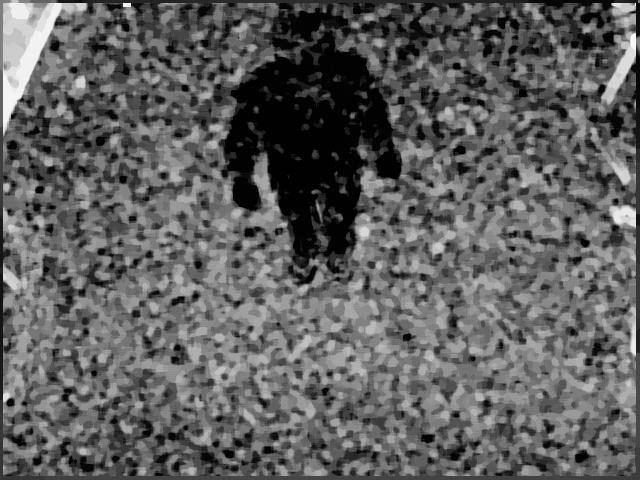
\includegraphics[width=.99\linewidth]{A3/lambda0.5.jpg}
		\caption{$\lambda=0.5$}
	\end{subfigure}
	\begin{subfigure}{.49\textwidth}
		\centering
		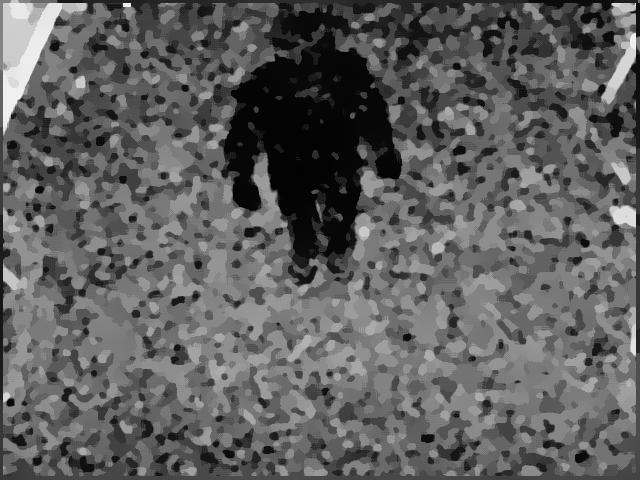
\includegraphics[width=.99\linewidth]{A3/lambda1.jpg}
		\caption{$\lambda=1$}
	\end{subfigure}
	\begin{subfigure}{.49\textwidth}
		\centering
		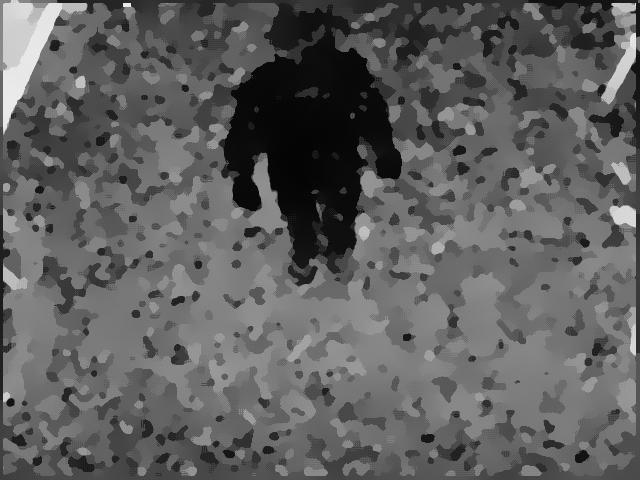
\includegraphics[width=.99\linewidth]{A3/lambda1.5.jpg}
		\caption{$\lambda=1.5$}
	\end{subfigure}
	\begin{subfigure}{.49\textwidth}
		\centering
		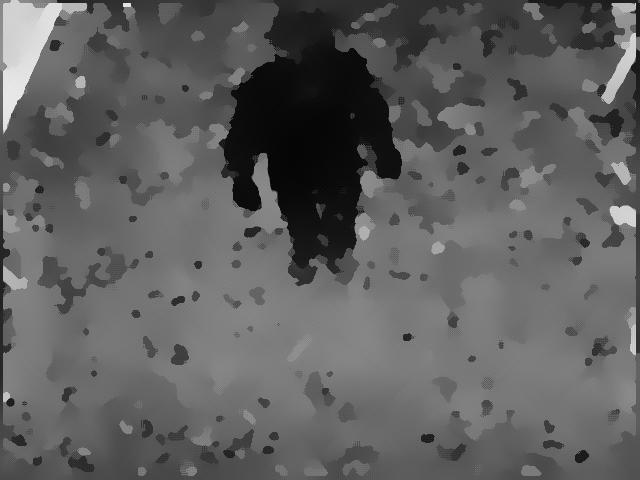
\includegraphics[width=.99\linewidth]{A3/lambda2.jpg}
		\caption{$\lambda=2$}
	\end{subfigure}

	\caption{Isotropes inhomogenes Diffusionsfilter mit $\epsilon_0=1$ und 500 Iterationen}
\end{figure}